% =========================================================== %
% UNINOVE: Modelo de trabalho acadêmico para tese (doutorado) %
% ou dissertação (mestrado) em conformidade com a             %
% ABNT NBR 14724:2011.                                        %
% Feito com base nos modelos da UNINOVE-PPGI e ICMC-USP       %
% Autor: André Luis Marques Ferreira dos Santos               %
% Programa de Doutorado em Administração (PPGA-UNINOVE)       %
% Atualização: 30/08/2021                                     %
% =========================================================== %
% configuração da fonte, pode ser courier ou times
\documentclass[courier]{uninove}
% -----------------------------------------------------------
% Pacotes adicionais
% -----------------------------------------------------------
\pgfplotsset{compat=1.17}     % resolve o problema do pacote pgfplots
\setlength{\headheight}{17pt} % resolve o problema do pacote Fancyhdr
\usepackage{epigraph}         % epígrafe
\usepackage{ragged2e}         % justificar texto nos agradecimentos
\usepackage{pdfpages}         % anexar pdfs
\usepackage{lastpage}		  % Usado pela Ficha catalográfica
% -----------------------------------------------------------
% pacote para lista de quadros
\DeclareCaptionType{quadro}
\usepackage[titletoc]{appendix}
\usepackage{trivfloat}
%\trivfloat{quadro}
\usepackage{multirow,tabularx}
%\usepackage[utf8]{inputenc}
%\usepackage{lipsum}
%\usepackage{graphicx}
\usepackage{float}            % pacote para colocar o caption no topo dos quadros
\floatstyle{plaintop}         % Coloca caption no topo
\newfloat{quadro}{htbp}{lop}  % Coloca caption no topo
\floatname{quadro}{Quadro}    % nome do caption
%\newcommand{\listofquadros}{\listof{quadro}{Lista de Quadros}} % renomeia o capítulo
\captionsetup[quadro]{listformat=simple}
\captionsetup{labelsep=endash} % muda ":" para "-" no caption dos quadros
\usepackage[justification=centering]{caption} % centraliza o caption nos quadros
% -----------------------------------------------------------
% pacotes para lista de equações
%\usepackage{tocbibind}
\usepackage{tocloft}    % também utilizado para alinhar sumário
%\usepackage{xpatch}
\usepackage{amsmath}
% -----------------------------------------------------------
% Habilitar lista de mapas
\DeclareCaptionType{mapa}
% -----------------------------------------------------------
% glossário (habilitar: B - D - E - F) .........................................
%\let\su@ExpandTwoArgs\relax        % A - resolve conflitos no pacote glossaries
%\let\IfSubStringInString\relax      % B - resolve conflitos no pacote glossaries
%\let\su@IfSubStringInString\relax  % C - resolve conflitos no pacote glossaries
%\usepackage[noredefwarn,xindy,translate=babel,nonumberlist,style=list,toc]{glossaries} % D
%\makeglossaries % E
%% ----------------------------------------- %
%	Glossário (preencher)
% ----------------------------------------- %

%\newglossaryentry{domain-knowledge}{%
%  name={domain knowledge},%
%  description={valid knowledge used to refer to an area of human endeavour, an autonomous computer activity, or other specialized discipline}}

%\newacronym{tla}{TLA}{Three Letter Acronym} % F
% -----------------------------------------------------------
% Índice remissivo
\usepackage{makeidx}
\makeindex

% Colocar hifens no sumario
\usepackage{titletoc}
\usepackage{chngcntr}
%.......................................................
% ---------------------------------------------- %
%                                                %
% Início do documento - comece a formatar daqui  %   
%                                                %
% ---------------------------------------------- %
%
\begin{document}
%
% ---------------------------------------------------------- %
%                                                            %
% Elementos pré-textuais                                     %
%                                                            %
% ---------------------------------------------------------- %
%
% Parâmetros para capa e folha de rosto
% (é necessário configurar todos)
%
\Universidade{UNIVERSIDADE NOVE DE JULHO - UNINOVE}
\Programa{PROGRAMA DE PÓS GRADUAÇÃO EM ADMINISTRAÇÃO - PPGA} 	
\Autor{NOME E SOBRENOME DO AUTOR}	 
\Titulo{TESE \& DISSERTAÇÃO -- UNINOVE (SP$\backslash$BRASIL):\\MODELO PARA MONOGRAFIAS DE MESTRADO E DOUTORADO.}
\Tipoexame{Qualificação}
\Titulacao{Doutor}
\Orientador{Dr. Nome do(a) Orientador(a) Vai Aqui}
\Coorientador{Dr. Nome do(a) Coorientador(a) Vai Aqui} % se não se aplica comentar em uninove-ppga.cls linha 376
\Ano{2021}
%
% ..........................................................
%
% Inputs (colocar comentários caso não se aplique)
%
% Capa
% ----------------------------------------- %
%	Capa (não mexer)
% ----------------------------------------- %
% gera a capa
\capa
% Folha de rosto
% ----------------------------------------- %
%	Folha de rosto (não mexer)
% ----------------------------------------- %
% gera a folha de rosto
\folharosto
% Errata
% ----------------------------------------- %
%	Errata (preencher)
% ----------------------------------------- %
\newpage
\textbf{ERRATA:}

De acordo com a NBR 14724:2011 é um elemento opcional.
É a lista inserida após a folha de rosto que descreve eventuais erros do texto
e suas respectivas correções, apresentada em folha avulsa acrescida ao
trabalho depois de impresso
Deve vir logo após a folha de aprovação.

\newpage
% Folha de aprovação
% ----------------------------------------- %
%	Folha de aprovação (não mexer)
% ----------------------------------------- %
% Após aprovação do trabalho a folha deve ser assinada, escaneada e
% incluída como abaixo:
\begin{folhadeaprovacao}
%\includepdf{folha-de-aprovacao-escaneada.pdf}
\includegraphics[page=1,width=0.9\linewidth,height=0.9\textheight]{material-de-apoio/pdfs/folha-de-aprovacao-escaneada.pdf}
\end{folhadeaprovacao}

\newpage
% Ficha catolográfica
% ----------------------------------------- %
%	Ficha catalográfica (não mexer)
% ----------------------------------------- %
%
% Inserir a ficha catalográfica em pdf
% ---
% Provavelmente a biblioteca da sua universidade lhe fornecerá um PDF
% com a ficha catalográfica definitiva após a defesa do trabalho. Quando estiver
% com o documento, salve-o como PDF no diretório do seu projeto e substitua todo
% o conteúdo de implementação deste arquivo pelo comando abaixo:
%
%\begin{fichacatalografica}
%\includepdf{ficha-catalografica.pdf}
%\end{fichacatalografica}
% ---
\setcounter{section}{0}
\renewcommand{\thesection}{\Alph{section}}
%\begin{minipage}{\textwidth} % usar opção para includepdf
\includegraphics[page=1,width=0.9\linewidth,height=0.9\textheight]{material-de-apoio/pdfs/ficha-catalografica.pdf}
%\includepdf[pages={1},scale=0.70]{material-de-apoio/pdfs/ficha-catalografica.pdf}
%\end{minipage}
% Dedicatória
% ----------------------------------------- %
%	Dedicatória (preencher)
% ----------------------------------------- %
\newpage
%\begin{dedicatoria}
\thispagestyle{empty}
   \vspace*{\fill}
   \centering
   \noindent
	\textbf{A dedicatória é opcional. Caso não deseje uma, deixar todo este
	arquivo em branco}.

   \textit{Este trabalho é dedicado às crianças adultas que,
   quando pequenas, sonharam em se tornar cientistas.} \vspace*{\fill}
%\end{dedicatoria}
\newpage
% Agradecimentos
% ----------------------------------------- %
%	Agradecimentos (preencher)
% ----------------------------------------- %

\newpage
\thispagestyle{plain}
\begin{center}
    \Large
    AGRADECIMENTOS
\end{center}

\justifying
A inclusão desta seção de agradecimentos é opcional, portanto, sua inclusão 
fica a critério do(s) autor(es), que caso deseje(em) fazê-lo deverá(ão) 
utilizar este espaço, seguindo a formatação de \textit{espaço simples e 
fonte padrão do texto (sem negritos, aspas ou itálico}.

\textbf{Caso não deseje utilizar os agradecimentos, deixar toda este arquivo
em branco}.

\newpage
% Epígrafe
% ----------------------------------------- %
%	Epígrafe (preencher)
% ----------------------------------------- %
\newpage
\setlength\epigraphwidth{.8\textwidth}
\setlength\epigraphrule{0pt}

\thispagestyle{empty}

\vspace*{\fill}
\epigraph{\itshape Begin at the beginning, the King said gravely, ``and go on till you come to the end: then stop.''}{---Lewis Carroll, \textit{Alice in Wonderland}}

\newpage
% Resumo
% ----------------------------------------- %
%	Resumo (preencher)
% ----------------------------------------- %
% Configuração do resumo e palavras-chave em Português

\PalavrasChave{UNINOVE, Dissertação, Doutorado, Mestrado, Estudo Único.}

\begin{resumo}

Com a finalidade de auxiliar a comunidade acadêmica, em particular os alunos de mestrado e doutorado, desenvolvi esse material.
Esse não é um material oficial da UNINOVE, porém foi desenvolvido com base no Manual de Trabalhos Acadêmicos da UNINOVE e normas da ABNT. Também utilizei o modelo desenvolvido pelo PPGI - UNINOVE e o modelo do ICMC-USP.
Por ser um trabalho voluntário e não ser um instrumento oficial da instituição recomendo antes de utilizar consultar a sua instituição para averiguar se segue as normas exigidas.
Apesar de ser feito com foco nos alunos da UNINOVE pode ser facilmente adaptado para outras instituições de ensino.
Por fim, é importante ressaltar que esse modelo é para dissertações "tradicionais" (as que utilizam estudo único). Para monografias com múltiplos estudos esse modelo não se aplica.

\end{resumo}
% Abstract
% ----------------------------------------- %
%	Abstract (preencher)
% ----------------------------------------- %
% configurações do resumo e palavras-chave em Inglês

\KeyWords{UNINOVE, Dissertation, Doctorate Degree, Mater Degree, Single Study.}

\begin{abstract}

With the purpose of helping the academic community, in particular the master and doctoral students, I developed this material.
This is not official UNINOVE material but was developed based on the UNINOVE Academic Works Manual and ABNT standards. I also used the model developed by PPGI - UNINOVE and the ICMC-USP model.
As it is voluntary work and is not an official instrument of the institution, I recommend that before using it to consult your institution to find out if it follows the required standards.
Despite being made with a focus on UNINOVE students, it can be easily adapted to other educational institutions.
Finally, it is important to emphasize that this model is for "traditional" dissertations (those that use a single study). For monographs with multiple studies, this model does not apply.

\end{abstract}
%
% ---------------------------
%
% Sumário
%
\tableofcontents 
\thispagestyle{empty}
\addtocontents{toc}{~\hfill\textbf{Páginas}\par}
\clearpage
% ---------------------------
%
% Listas
%
% comentar listas que não se aplicaram ao modelo
% Lista de figuras
% ----------------------------------------- %
%	Lista de figuras (não mexer)
% ----------------------------------------- %

\cftsetindents{figure}{0em}{5.0em}
\renewcommand{\cftfigpresnum}{Figura }
%\renewcommand{\cftfigaftersnum}{ -- }
\renewcommand\cftfigaftersnum{\enspace--\enspace}
\counterwithout{figure}{chapter} % conta sem o número do capítulo
\listoffigures
\thispagestyle{empty}

\newpage
% Lista de algoritmos
% ----------------------------------------- %
%	Lista de algoritmos (não mexer)
% ----------------------------------------- %

\addcontentsline{toc}{chapter}{Lista de Algoritmos}

\let\oldlistofalgorithms\listofalgorithms
\let\oldnumberline\numberline% Store \numberline
\newcommand{\algnumberline}[1]{Algoritmo~#1 -- }
\renewcommand{\listofalgorithms}{%
  \let\numberline\algnumberline% Update \numberline
  \oldlistofalgorithms
  \let\numberline\oldnumberline% Restore \numberline
}

\listofalgorithms
\thispagestyle{empty}


% Lista de equações
% ----------------------------------------- %
%	Lista de equações (não mexer)
% ----------------------------------------- %
\newcommand{\listequationsname}{Lista de Equações}

\newlistof{myequations}{equ}{\listequationsname}
\newcommand{\myequations}[1]{%
\addcontentsline{equ}{myequations}{Equação \protect\numberline{\theequation  \enspace--\enspace}#1}\par}
\setlength{\cftmyequationsnumwidth}{2em}
\xpretocmd{\listofmyequations}{\addcontentsline{toc}{chapter}{\listequationsname}}{}{}
\counterwithout{equation}{chapter} % conta sem o número do capítulo

\listofmyequations


%\listofmyequations
% Lista de quadros
% ----------------------------------------- %
%	Lista de quadros (não mexer)
% ----------------------------------------- %

\renewcommand{\cftfigpresnum}{Quadro\ }
\newlength{\mylenf}
\settowidth{\mylenf}{\cftfigpresnum}
\setlength{\cftfignumwidth}{\dimexpr\mylenf+3em}
\renewcommand\cftfigaftersnum{\enspace--\enspace}
%\renewcommand{\cfttabaftersnum}{ -- }

\renewcommand{\listquadroname}{Lista de Quadros}
\counterwithout{quadro}{chapter} % conta sem o número do capítulo

\listofquadro

%\listofquadros
% Lista de abreviaturas e siglas
% --------------------------------------------------------- %
%	Lista de Abreviaturas (preencher conforme necessidade)
% --------------------------------------------------------- %
% lista de abreviaturas (não colocar espaçamentos adicionais, pois eles constam dentro do environment)

\begin{listaabreviaturas}%
	MM & Morfologia matemática \\
	CC & Componente conexo \\
	EE & Elemento estruturante \\
	MS & Mumford-Shah \\
	\textit{poset} &  Acrônimo para a expressão em inglês \textit{partially ordered set}\\
				   &  (em português: conjunto parcialmente ordenado) \\
	\textit{pixel} &  Acrônimo para a expressão em inglês \textit{picture element}\\
				   &  (em português: elemento da imagem)
\end{listaabreviaturas}

\newpage
% Lista de tabelas
% ----------------------------------------- %
%	Lista de tabelas (não mexer)
% ----------------------------------------- %

\cftsetindents{table}{0em}{5.0em}
\renewcommand\cfttabpresnum{Tabela }
%\renewcommand{\cfttabaftersnum}{ -- }
\renewcommand\cfttabaftersnum{\enspace--\enspace}
\counterwithout{table}{chapter}  % conta sem o número do capítulo

\listoftables
\cleardoublepage

\newpage
% Lista de símbolos
% ---------------------------------------------------- %
%	Lista de Símbolos (preencher conforme necessidade)
% ---------------------------------------------------- %
% lista de símbolos (não colocar espaçamentos adicionais, pois eles contam dentro do environment)
% atualmente a lista não suporta múltiplas páginas, ou seja ela quebra a lista inteira.

\begin{listasimbolos}%
	\simbolos{Conceitos básicos} {%		
		$ \mathbb{Z} $ & Conjunto dos números inteiros \\						
		$ \mathbb{N} $ & Conjunto dos números naturais \\		
		$ \mathbb{R}^+ $ & Conjunto	dos números reais positivos \\	 		
	}
	\simbolos{Imagens} {%	
		$ f $ & Váriavel que representa uma imagem \\			
		$ \mathcal{D} $ & Conjunto que representa o domínio da imagem \\					
		$ \mathbb{K} $ & Conjunto que representa o contradomínio da imagem \\		
	}
\end{listasimbolos}

\newpage
% Lista de mapas
% ----------------------------------------- %
%	Lista de Mapas (não mexer)
% ----------------------------------------- %
\renewcommand{\cftfigpresnum}{Mapa\ }
%\newlength{\mylenf}
\settowidth{\mylenf}{\cftfigpresnum}
\setlength{\cftfignumwidth}{\dimexpr\mylenf+2.0em}
\renewcommand\cftfigaftersnum{\enspace--\enspace}
%\renewcommand{\cfttabaftersnum}{ -- }
\counterwithout{mapa}{chapter}  % conta sem o número do capítulo
\renewcommand{\listmapaname}{Lista de Mapas}
\newlistentry{map}{lom}{0}
\listofmapas

\newpage
%
% CORPO DO DOCUMENTO
%
% ---------------------------------------------------------- %
%                                                            %
% Elementos textuais                                         %
%                                                            %
% ---------------------------------------------------------- %
%
% Introdução
% ----------------------------------------- %
%	Capítulo Introdução (preencher)
% ----------------------------------------- %
\chapter{Introdução}\label{chp:20_introducao}
% ============================================================
% comando para customizar o número das seções (não mexer)
\renewcommand{\thesection}{\arabic{chapter}.\arabic{section}}
% ============================================================

\begin{resumocapitulo}
As seções e subseções são configuradas de acordo com a norma ABNT adotada pela UNINOVE (tamanho da fonte, espaçamento...). As numerações de página estão alinhadas a direita no \textit{header}.
\end{resumocapitulo}

Introdução é a parte inicial do texto que deve apresentar o assunto, elementos essenciais e metodologia aplicada para o desenvolvimento do trabalho.

É importante que o texto seja redigido de forma clara e desperte o interesse do leitor. Recomenda-se que seja a última parte a ser escrita no trabalho.
% Revisão da Literatura
% ------------------------------------------ %
%  Capítulo Revisão da Literatura (preencher)
% ------------------------------------------ %
\chapter{Referencial Teórico}\label{chp:21_literatura}
% ============================================================
% comando para customizar o número das seções (não mexer)
%\renewcommand{\thesection}{\arabic{chapter}.\arabic{section}}
% ============================================================

\begin{resumocapitulo}
As seções e subseções são configuradas de acordo com a norma ABNT adotada pela UNINOVE (tamanho da fonte, espaçamento...). As numerações de página estão alinhadas a direita no \textit{header}.
\end{resumocapitulo}

A revisão bibliográfica, ou revisão da literatura, é uma análise meticulosa e ampla das publicações correntes em uma determinada área do conhecimento. Segundo o Manual de produção de textos acadêmicos e científicos, "As pesquisas de revisão bibliográfica (ou revisão de literatura) são aquelas que se valem de publicações científicas em periódicos, livros, anais de congressos etc., não se dedicando à coleta de dados in natura, porém não configurando em uma simples transcrição de ideias. Para realizá-la, o pesquisador pode optar pelas revisões de narrativas convencionais ou pelas revisões mais rigorosas \cite{wiki:xxx}.

% Metodolodia
% ----------------------------------------- %
%	Capítulo Metodologia (preencher)
% ----------------------------------------- %
\chapter{Metodologia}\label{chp:22_metodologia}
% ============================================================
% comando para customizar o número das seções (não mexer)
%\renewcommand{\thesection}{\arabic{chapter}.\arabic{section}}
% ============================================================

\begin{resumocapitulo}
A metodologia é o estudo dos métodos. Isto é, o estudo dos caminhos para se chegar a um determinado fim. Com o objetivo de analisar as características dos vários métodos indispensáveis tais como: avaliar capacidades, limitações e criticar os pressupostos quanto sua utilização.
\end{resumocapitulo}

% Resultados
% ----------------------------------------- %
%	Capítulo Resultados (preencher)
% ----------------------------------------- %
\chapter{Resultados}\label{chp:23_resultados}
% ============================================================
% comando para customizar o número das seções (não mexer)
%\renewcommand{\thesection}{\arabic{chapter}.\arabic{section}}
% ============================================================

\begin{resumocapitulo}
Coloque neste capítulo os resultados da pesquisa.
\end{resumocapitulo}
% Conclusão
% ----------------------------------------- %
%	Capítulo Conclusão (preencher)
% ----------------------------------------- %
\chapter{Conclusão}\label{chp:24_conclusao}
% ============================================================
% comando para customizar o número das seções (não mexer)
%\renewcommand{\thesection}{\arabic{chapter}.\arabic{section}}
% ============================================================

\begin{resumocapitulo}
Coloque neste capítulo as considerações finais da pesquisa.
\end{resumocapitulo}
% Capítulo com exemplos (comentar essa linha para não exibir)
% ----------------------------------------- %
%	Capítulo Exemplo (faça testes aqui)
% ----------------------------------------- %
% ============================================================
% comando para customizar o número das seções (não mexer)
%\renewcommand{\thesection}{\arabic{chapter}.\arabic{section}}
% ============================================================
% Use esse capítulo para testes. Depois comente esse
% arquivo em "principal.tex" para não ser exibido no
% documento final.

\chapter{Capítulo Exemplo}\label{chp:exemplos}

\begin{resumocapitulo}
Esse é apenas um capítulo de demonstração. Inserir alguns comandos em \LaTeX{} para desenvolvimento deste modelo. Não há necessidade de deletar o material que está neste capítulo, apenas vá no arquivo \texttt{principal.tex} e comente ( coloque o símbolo: \%) na linha onde está o nome do arquivo que representa esse capítulo (\texttt{exemplo.tex}).
\end{resumocapitulo}

%-------------------------- %
% Glossário                 %
%-------------------------- %
\section{Como habilitar glossário}

\begin{enumerate}
    \item No preambulo do arquivo {\color{red}$\backslash$\texttt{principal.tex}} (em: \% glossário...) habilitar:
    \begin{enumerate}
        \item IfSubStringInString
        \item usepackage\{glossaries\}
        \item makeglossaries
        \item 31\_glossario
    \end{enumerate}
    \item No corpo do arquivo {\color{red}$\backslash$\texttt{principal.tex}} (procurar no final da página) habilitar:
    \begin{enumerate}
        \item $\backslash$printglossaries
    \end{enumerate}
    \item No arquivo {\color{red}\texttt{31\_glossario.tex}}:
    \begin{enumerate}
        \item Escreva as entradas (expressões) para o glóssario.
        \item siga o exemplo da página ou acesse a \hyperlink{https://pt.overleaf.com/learn/latex/Glossaries}{página no Overleaf} para maiores detalhes.
        \item {\color{red}Atenção:} coloque primeiro a expressão no Glossário (arquivo: 31\_glossario.tex) antes de usar no texto principal.
    \end{enumerate}
\end{enumerate}

\subsection{Exemplo de como usar termos do Glossário}

%The \texttt{glossaries} package automatically generates a list of glossary entries. It's great for keeping track of your \gls{domain-knowledge} and \glspl{tla}. In this example we've put the glossary definitions in a separate \texttt{glossary.tex} file, which you can edit via the project menu.

%---------------------------------------------------------------
\newpage
%-------------------------- %
% Notas de rodapé           %
%-------------------------- %
\section{Notas de rodapé}
Esse documento foi desenvolvido com base no modelo do PPGI-UNINOVE\footnote{Universidade Nove de Julho}, de autoria de Charles Ferreira Gobber.
É uma extensão do template do IME-USP\footnote{Instituto de Matemática e Estatística} desenvolvido pelo professor Jesús P. Mena-Chalco.

\textit{Para saber mais sobre nota de rodapé acesse \hyperlink{https://pt.overleaf.com/learn/latex/Footnotes}{Overleaf}}.
%-------------------------- %
% Hierárquia de seções      %
%-------------------------- %
\section{Hierarquia de seções}
\begin{itemize}
    \item $\backslash$chapter{}
    \begin{itemize}
        \item $\backslash$section{}
        \begin{itemize}
            \item $\backslash$subsection{}
            \begin{itemize}
                \item $\backslash$subsubsection{}
            \end{itemize}
        \end{itemize}
    \end{itemize}
\end{itemize}

%---------------------------------------------------------------
\newpage
%-------------------------- %
% Figuras                   %
%-------------------------- %
\section{Exemplo de figuras}
Consideram-se figuras os desenhos, mapas, esquemas, gráficos, fórmulas, modelos, fotografias, diagramas, fluxogramas, organogramas, entre outros.

Pelas normas da ABNT as figuras devem ser adicionadas com um título em cima e a fonte em baixo. Depois deve ser referenciada no texto o mais próximo possível. \textbf{Todas figuras inseridas devem ser referenciadas}, por exemplo (Figura~\ref{fig:estr_trab_academicos}).
Neste documento, organize as figuras na pasta \texttt{figuras}.
% Figura 1 ............................................................

\begin{figure}[htbp]
\hypertarget{arquitetura}{%
\caption{Estrutura de Trabalhos Acadêmicos}\label{fig:estr_trab_academicos}
\begin{center}
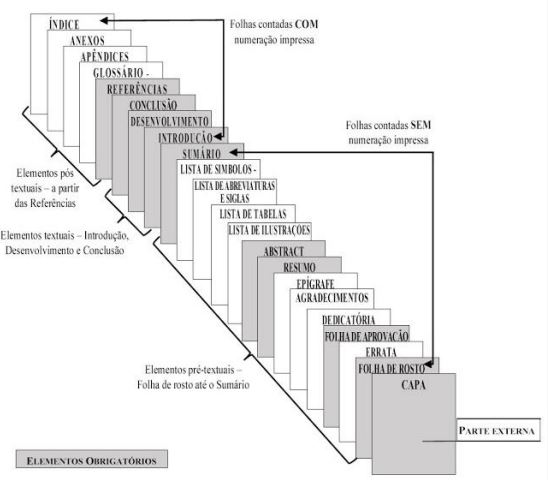
\includegraphics{material-de-apoio/figuras/estrutura_monografias.JPG}\\
\fonte{Manual de Trabalhos Acadêmicos UNINOVE}
\end{center}
}
\end{figure}

Maiores detalhes de como customizar figuras, inserir figuras no meio do texto, rotacionar etc consultar os materiais:
\begin{itemize}
    \item \hyperlink{https://www.ime.unicamp.br/~marchesi/Allegati/NotasdeAulaLaTeX.pdf}{IMEC-UNICAMP Notas de Aula \LaTeX{}}, página 26.
    \item \hyperlink{http://www.uel.br/projetos/matessencial/superior/pdfs/latexmat.pdf}{\LaTeX{} para Matemática - Departamento de Matemática UEL}, página 60.
\end{itemize}
%---------------------------------------------------------------
\newpage
%-------------------------- %
% Equações                  %
%-------------------------- %
\section{Exemplo de expressões matemáticas}

% Equação exemplo .........................................................
% Exemplo de equação
\begin{equation}\label{eq:Eq1}
   a=b
\end{equation}
\myequations{Equation number \ref{eq:Eq1}}


Equação~\ref{eq:Eq1}

%-----------------------------
\begin{itemize}
    \item \textbf{Sites interessantes para expressões e símbolos matemáticos:}
    \begin{itemize}
        \item \hyperlink{https://pt.overleaf.com/learn/latex/Mathematical_expressions}{Mathematical expressions - Overleaf.}
        \item \hyperlink{http://tug.ctan.org/info/short-math-guide/short-math-guide.pdf}{Short Math Guide for \LaTeX{}}
        \item \hyperlink{http://www.ams.org/arc/tex/amsmath/amsldoc.pdf}{User's Guide for the \texttt{amsmath} Package}
        \item \hyperlink{https://www.ime.unicamp.br/~marchesi/Allegati/NotasdeAulaLaTeX.pdf}{IMEC-UNICAMP Notas de Aula \LaTeX{}}
    \end{itemize}
\end{itemize}

%---------------------------------------------------------------
\newpage
%-------------------------- %
% Quadros e tabelas         %
%-------------------------- %
% Exemplo de quadro ..............................................
\section{Exemplo de quadro e tabela}
Quadros são formados por linhas verticais e horizontais, deem ter todas extremidades fechadas e, geralmente, são utilizados para \textbf{dados qualitativos}.

A diferença do quadro pra tabela é que o quadro tem linhas verticais.
Quadro~\ref{quad:exemplo_de_quadro}

% Exemplo de quadro

\begin{quadro}[!ht]
%\caption{Quadro de Exemplo}\label{quad:exemplo_de_quadro}
\caption{\label{quad:exemplo_de_quadro}Quadro de Exemplo}
\centering
\begin{tabular}{ |p{3cm}||p{3cm}|p{3cm}|p{3cm}|  }
\hline
\multicolumn{4}{|c|}{Country List} \\
\hline
Country & ISO ALPHA 2 & ISO ALPHA 3 & ISO Code\\
\hline
Afghanistan   & AF    &AFG&   004\\
Aland Islands&   AX  & ALA   &248\\
Albania &AL & ALB&  008\\
Algeria    &DZ & DZA&  012\\
American Samoa&   AS  & ASM&016\\
Andorra& AD  & AND   &020\\
Angola& AO  & AGO&024\\
\hline
\end{tabular}
\vskip 0.2cm
\fonte{Adaptado de \hyperlink{https://pt.overleaf.com/learn/latex/Tables}{Overleaf}}
\end{quadro}
\vspace{0em}
\footnotesize Se usar o comando \texttt{fonte} dentro do ambiente da tabela a "fonte" fica centralizada, caso contrário fica fora.

\begin{itemize}
    \item Para maiores detalhes de como fazer quadros veja:
    \begin{itemize}
        \item \hyperlink{https://wp.ufpel.edu.br/diehl/files/2017/06/aula11_ccf.pdf}{Comunicação Científica em Física}.
    \end{itemize}
\end{itemize}

\hrulefill

% Exemplo de tabela ..............................................
Enquanto os quadros são fechados e apresentam dados qualitativos,
as tabelas são abertas e apresentam dados estatísticos numéricos.
Linhas horizontais só se admitem no cabeçalho e no rodapé.
\begin{itemize}
    \item \textbf{Não deve figurar dados em branco:}
    \begin{itemize}
        \item Traço indica dado inexistente
        \item Reticências indicam dado desconhecido
        \item Zero deve ser usado quando o dado for menor que a metade da unidade adotada para a expressão do dado
    \end{itemize}
\end{itemize}

A ilustração a seguir (Tabela~\ref{quad:exemplo_de_quadro}) é um exemplo de quadro, pelas normas da ABNT.
% Exemplo de tabela
% Fonte: http://www1.maths.leeds.ac.uk/LaTeX/TableHelp1.pdf
\begin{table}[h]
\label{tab:exemplo}
\caption{Tabela de Exemplo} % title name of the table
\centering % centering table
\begin{tabular}{l c c rrrrrrr} % creating 10 columns
\hline\hline % inserting double-line
 Audio &Audibility & Decision &\multicolumn{7}{c}{Sum of Extracted Bits}
\\ [0.5ex]
\hline % inserts single-line
% Entering 1st row
 & &soft &1 & $-1$ & 1 & 1 & $-1$ & $-1$ & 1 \\[-1ex]
\raisebox{1.5ex}{Police} & \raisebox{1.5ex}{5}&hard
& 2 & $-4$ & 4 & 4 & $-2$ & $-4$ & 4 \\[1ex]
% Entering 2nd row
& &soft & 1 & $-1$ & 1 & 1 & $-1$ & $-1$ & 1 \\[-1ex]
\raisebox{1.5ex}{Beethoven} & \raisebox{1.5ex}{5}& hard
&8 & $-8$ & 2 & 8 & $-8$ & $-8$ & 6 \\[1ex]
% Entering 3rd row
& &soft & 1 & $-1$ & 1 & 1 & $-1$ & $-1$ & 1 \\[-1ex]
\raisebox{1.5ex}{Metallica} & \raisebox{1.5ex}{5}& hard
&4 & $-8$ & 8 & 4 & $-8$ & $-8$ & 8 \\[1ex]
% [1ex] adds vertical space
\hline % inserts single-line
\end{tabular}
\vskip 0.2cm
\fonte{Adaptado de \hyperlink{http://www1.maths.leeds.ac.uk/LaTeX/TableHelp1.pdf}{Creating Tables with \LaTeX{}}}
\end{table}

%---------------------------------------------------------------
\newpage
%-------------------------- %
% Mapas                     %
%-------------------------- %
\section{Exemplo de mapas}
Inserir o mais próximo do texto a que se referem.
No topo da imagem inserir o título.
Centralizar imagem, título, legenda e fonte.
Utilizar fonte 10.
Na parte inferior citar a fonte (mesmo que seja o próprio autor).

O Mapa~\ref{map:brasil_mapa} representa as UFs do Brasil.

\begin{mapa}[H]
\centering
\caption{Mapa do Brasil}\label{map:brasil_mapa}
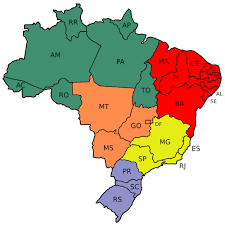
\includegraphics[scale=0.9]{material-de-apoio/mapas/mapa-do-brasil.png}\\
\fonte{Google}
\end{mapa}

%---------------------------------------------------------------
\newpage
%-------------------------- %
% Algoritmos                %
%-------------------------- %

Exemplo de pseudocódigo utilizando o pacote {\color{red}algorithm2e}:

% Exemplo de algoritmo:
% controla endentação
\begin{algorithm}[H]
\SetAlgoLined
\Entrada{$S,\eta, U$} 
\Saida{Número esperado de nós atingidos}
\Inicio{
	$\sigma(S) = 0$ \\
\Para{cada $u \in S$}{
	$\sigma(S)\leftarrow \sigma(S)+\textsc{Backtrack}(u,\eta,W,U)$\\
}
}
\Retorna{$\sigma(S)$}
\label{alg1}
\caption{\textsc{Esperança}}
\end{algorithm}

%---------------------------------------------------------------
\newpage
%-------------------------- %
% Índice Remissivo          %
%-------------------------- %
\section{Exemplo de Índice Remissivo}
Para criar um índice remissivo devemos usar o pacote \texttt{makeidx} e dar o comando
\texttt{$backslash$makeindex} no preâmbulo do documento para inicializá-lo.

Cada entrada do índice é adicionada logo após a ocorrência da mesma da seguinte forma:

$backslach$\{chave\}, onde a \textit{chave} é o texto que aparecerá no índice (com a página correspondente). Se uma mesma chave aparecer mais de uma vez no texto ela aparecerá uma única vez no índice, com os números das páginas das ocorrências. É possível incluir suentradas e s subsubentradas de uma entrada colocando "\!" entre elas.

Para maiores detalhes acesse o documento online: \hyperlink{https://www.ime.usp.br/~viviane/MAP2212/minicurso.pdf}{Minicurso de \LaTeX{}}.
Ou \hyperlink{https://netsgo.wordpress.com/2010/09/28/aprenda-a-criar-um-indice-remissivo-no-latex-learning-how-to-create-an-index-with-latex/}{Aprenda a criar um índice remissivo no \LaTeX{}}.

Exemplo:
\begin{itemize}
    \item \index{Amplificador ótico} é um equipamento responsável por amplificar o sinal óptico proveniente do transmissor de vídeo.
    \item \index{Amplificaro ótico!EDFA} do inglês \textit{Erbium Doped Fiber Amplifier}.
\end{itemize}
%
% ---------------------------------------------------------- %
%                                                            %
% Elementos pós textuais                                     %
%                                                            %
% ---------------------------------------------------------- %
%
% ---------------------------
% Bibliografia
\bibliography{referencias}
% ---------------------------
% Glossário
%% ----------------------------------------- %
%	Glossário (preencher)
% ----------------------------------------- %

%\newglossaryentry{domain-knowledge}{%
%  name={domain knowledge},%
%  description={valid knowledge used to refer to an area of human endeavour, an autonomous computer activity, or other specialized discipline}}

%\newacronym{tla}{TLA}{Three Letter Acronym} (habilitar apenas para entradas manuais)
%\printglossaries
% ---------------------------
% Apêndices
% -------------------------------------------- %
%	Apêndices (configurar em arquivo externo)
% -------------------------------------------- %
% Etapas:
% 1. Criar um arquivo ".tex" na pasta "\material-de-apoio\apendices".
% 2. Configurar arquivo da etapa 1.
% 3. Neste arquivo ("apendices.tex") copiar estrutura do "Apêndice A".

% Apêndice A ..................................................
\begin{appendices}
\chapter{}
% ------------------------------------------- %
%	Apêndice A (alterar conforme necessidade)
% ------------------------------------------- %

De acordo com a NBR 14724:2011 é um elemento opcional. É o texto ou documento elaborado pelo autor, a fim de complementar sua argumentação. Deve ser apresentado em folha própria com numeração contínua à do texto principal, na qual deve ser colocado a palavra Apêndice em letra maiúscula e a letra de identificação, seguidos de travessão e em letra minúscula o título do apêndice.
\clearpage
\newpage
\end{appendices}
\newpage

% Apêndice B ..................................................
\begin{appendices}
\chapter{}
% ------------------------------------------- %
%	Apêndice B (alterar conforme necessidade)
% ------------------------------------------- %
% Inserir a primeira página do pdf (procedimento necessário para não ficar com página em branco)
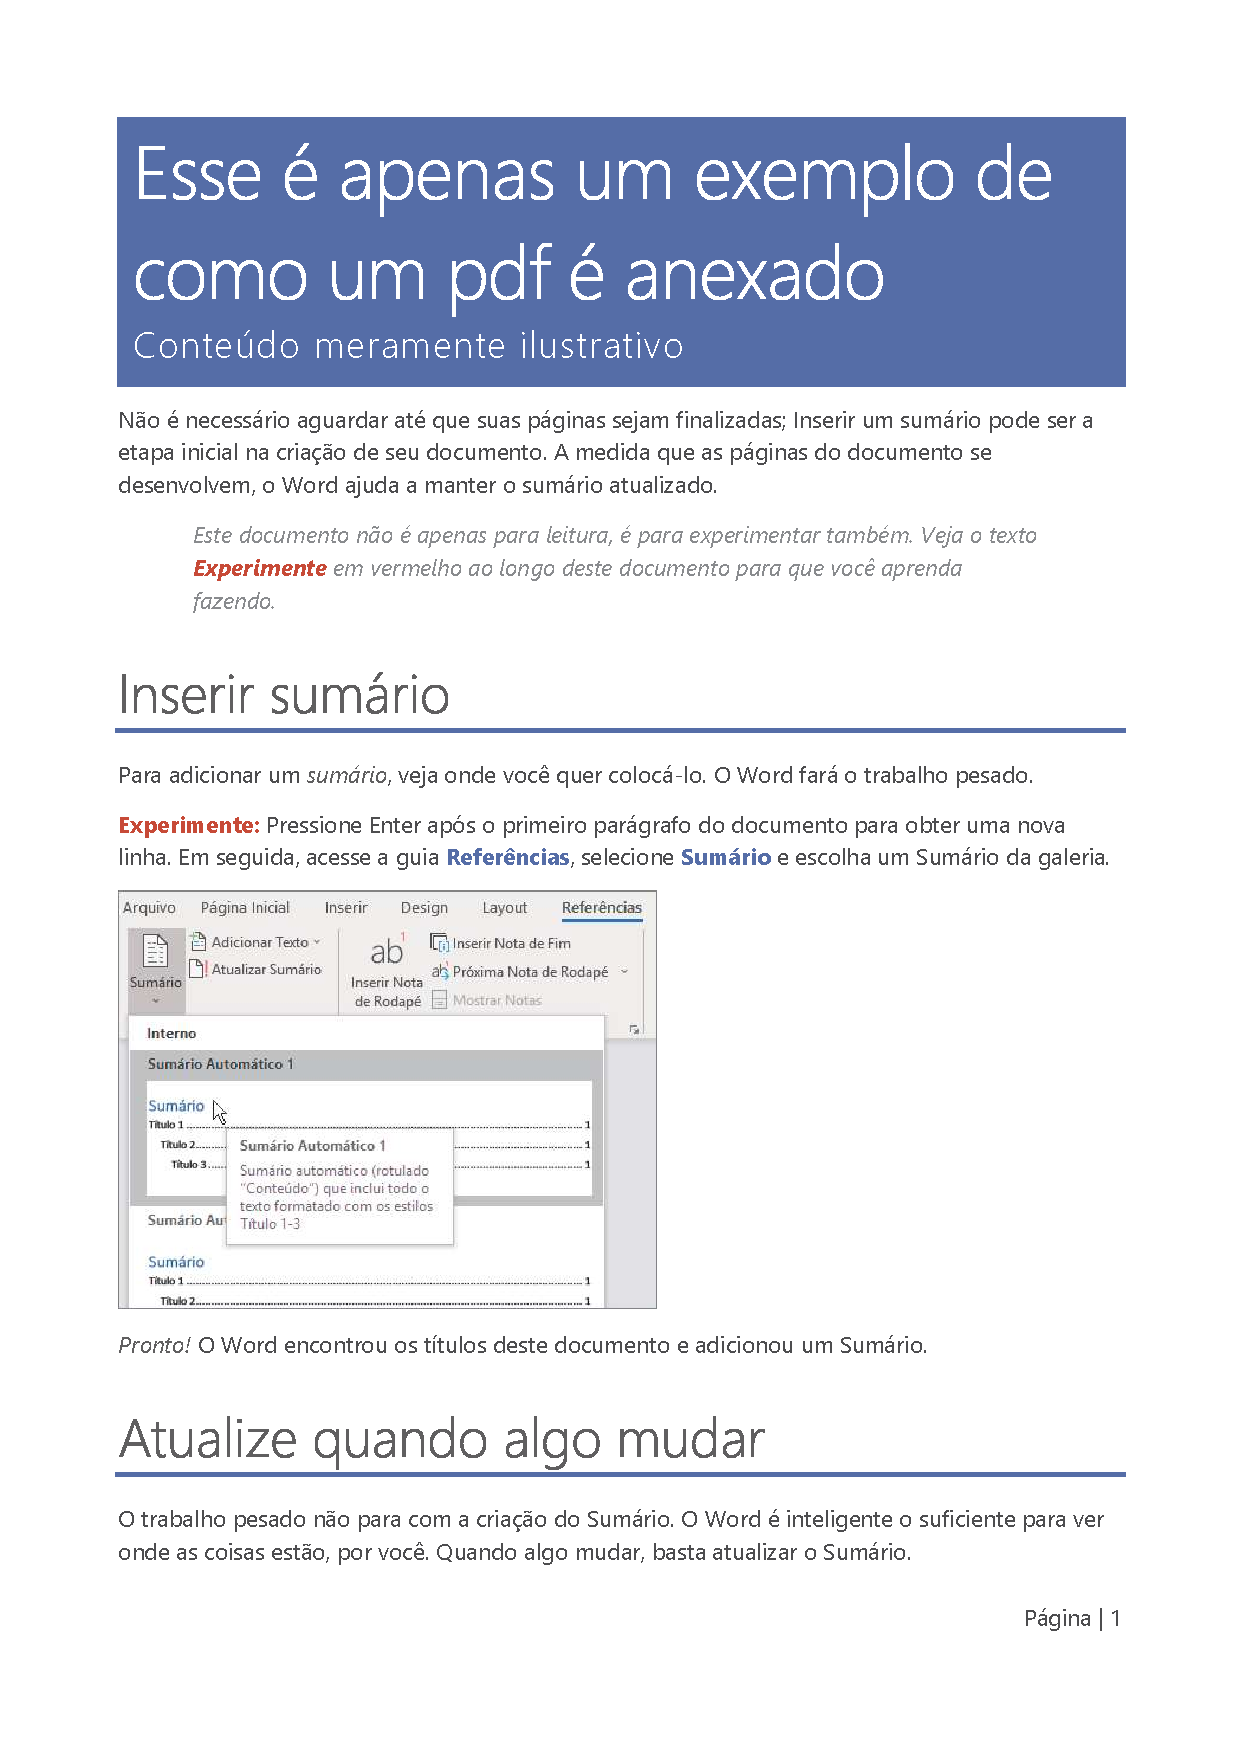
\includegraphics[page=1,width=0.9\linewidth,height=0.9\textheight]{material-de-apoio/pdfs/storopoli-et-al_2021_Simulation-Driven_COVID-19.pdf}

% Inserir demais páginas do pdf
\includepdf[pages={2-},scale=0.80,pagecommand={}]{material-de-apoio/pdfs/storopoli-et-al_2021_Simulation-Driven_COVID-19.pdf}

\newpage
\end{appendices}
\newpage
% Anexos
% ----------------------------------------- %
%	Anexos (não mexer)
% ----------------------------------------- %

% Anexo A ..................................................
\begin{appendix}
\chapter*{Anexo A}% If \appendix doesn't insert a \chapter
\addcontentsline{toc}{chapter}{Anexo A}% Print Appendix in ToC
% ------------------------------------------- %
%	Anexo A (alterar conforme necessidade)
% ------------------------------------------- %
De acordo com a NBR 14724:2011 é um elemento opcional. É o texto ou documento não
elaborado pelo autor, que contribui para fundamentação, comprovação e ilustração do trabalho.
Deve ser apresentado em folha própria com numeração contínua à do texto principal, na qual
deve ser colocado a palavra Anexo em letra maiúscula e a letra de identificação, seguidos de
travessão e em letra minúscula o título do anexo.
\end{appendix}
\newpage

% Anexo B ..................................................
\begin{appendix}
\chapter*{Anexo B}% If \appendix doesn't insert a \chapter
\addcontentsline{toc}{chapter}{Anexo B}% Print Appendix in ToC
% ------------------------------------------- %
%	Anexo B (alterar conforme necessidade)
% ------------------------------------------- %

% Inserir a página selecionada do pdf (procedimento necessário para não ficar com página em branco)
\includegraphics[page=26,width=0.9\linewidth,height=0.9\textheight]{material-de-apoio/pdfs/Manual_de_Trabalhos_Academicos_ABNT_UNINOVE.pdf}

% Inserir demais páginas do pdf
%\includepdf[pages={2-},scale=0.80,pagecommand={}]{material-de-apoio/pdfs/Manual_de_Trabalhos_Academicos_ABNT_UNINOVE.pdf}

\newpage
\end{appendix}
\newpage
% Índice
% ----------------------------------------- %
%	Índice Remissivo (não mexer)
% ----------------------------------------- %

\printindex
%
\end{document}
% =========================================================== %
% ----------------------------------------------------------- %
% .................... FIM DO DOCUMENTO ..................... %
% ----------------------------------------------------------- %
% =========================================================== %